\section{Data analysis}

All but one measurements were done on the same measuring rail as seen in figure \ref{fig::rail}, with an included \si{\milli \m}-scale. 
\begin{figure}[h!]
	\centering
	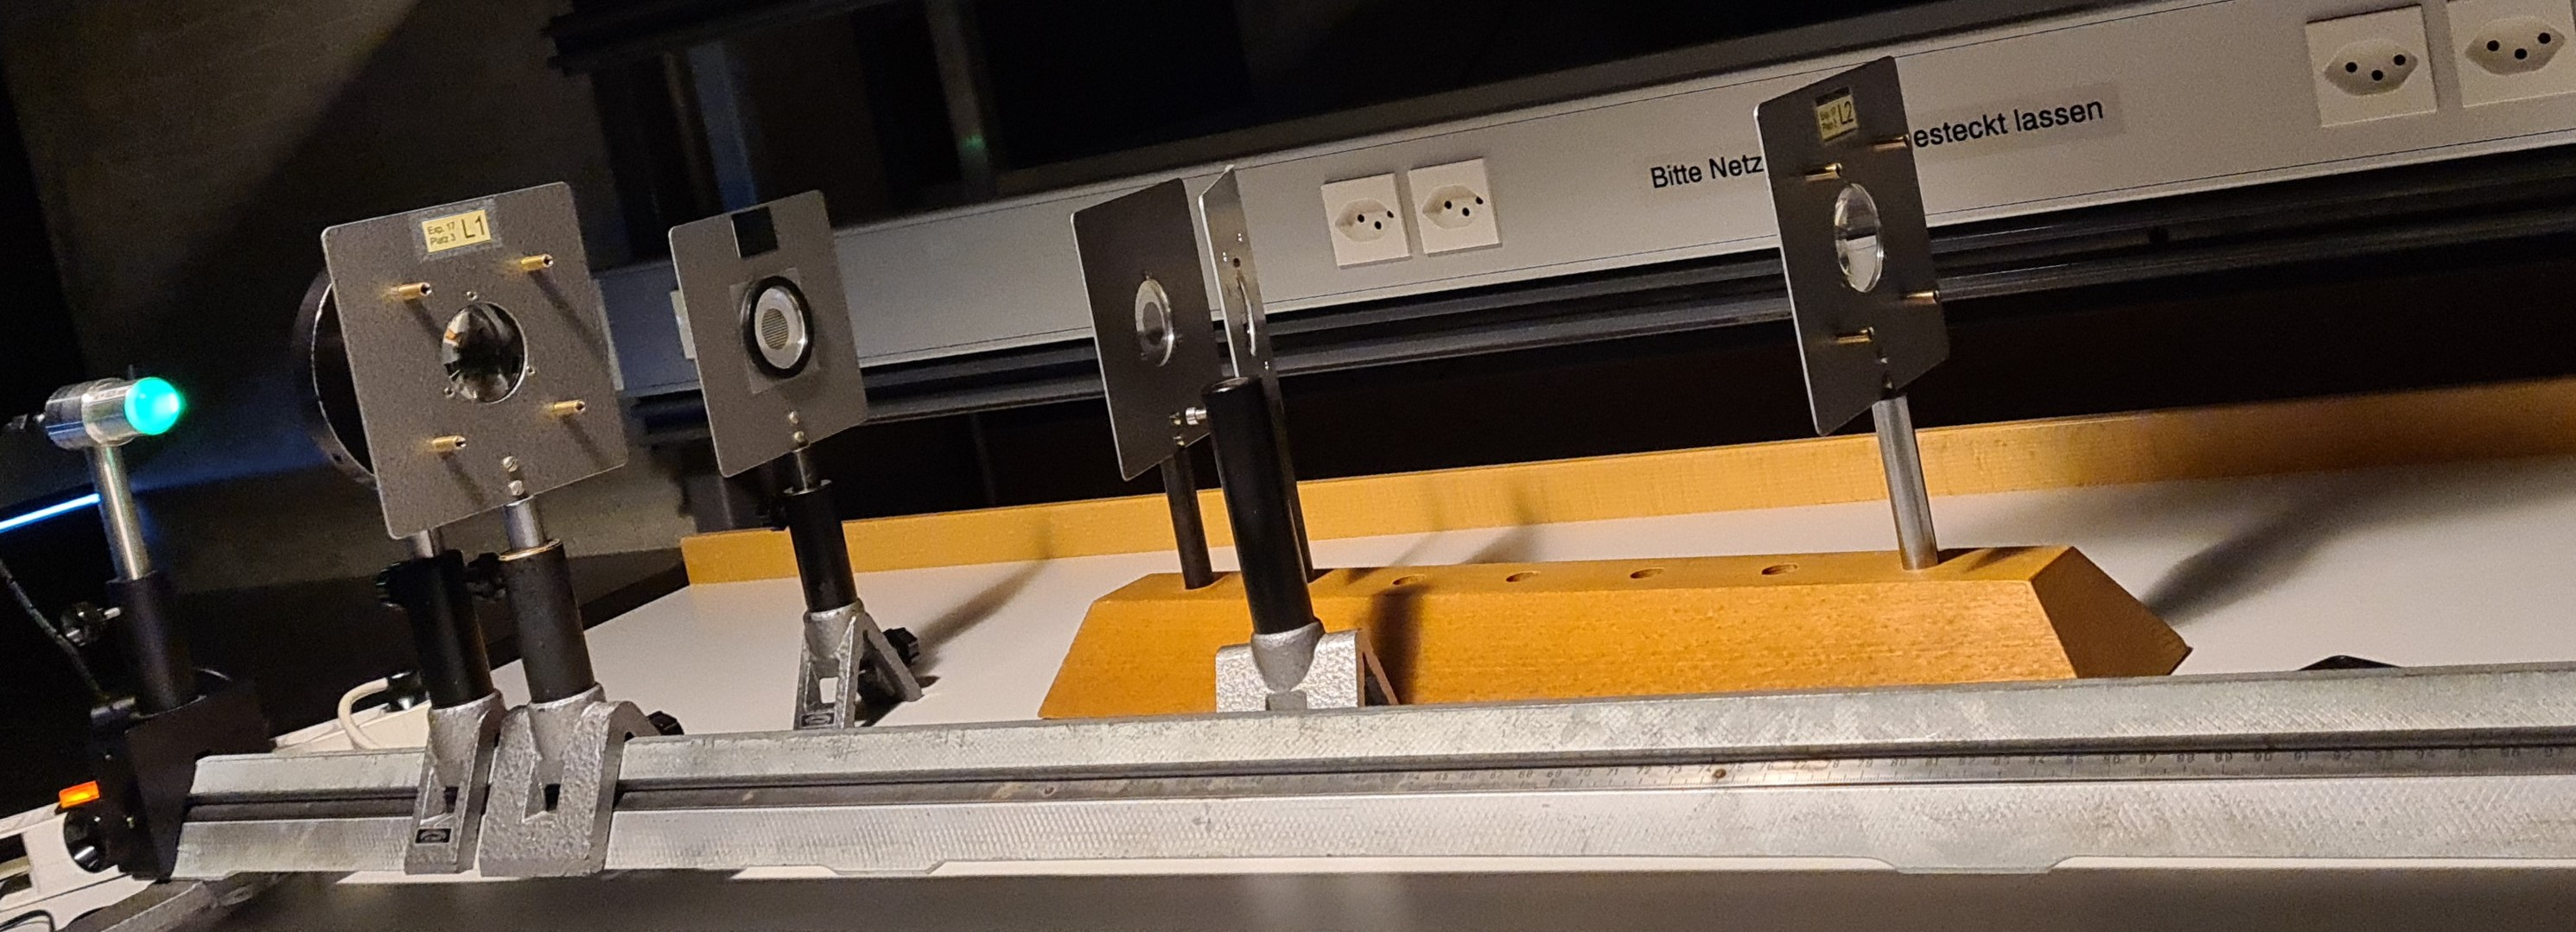
\includegraphics[width=\textwidth]{img/railcut.jpeg}
	\caption{Photo of the measurement rail, light source (left) and the setup from the critical slit width experiment from section \ref{chap::slit}.}
	\label{fig::rail}
\end{figure}

Since the later described error of focusing is way bigger, the following smaller sources are included in the focusing error.
In a setup with a \si{\milli \m} measuring rail like in figure \ref{fig::rail}, the best reading accuracy is $\pm 0.25 \si{\milli \m}$. 
If well done the parallax error can be included in this error margin, otherwise the parallax error can be added on top.
Depending on rail length and material a certain temperature error has to be included. 
Since the coefficient of length expansion for most metals used in length measuring devices is in the magnitude of $10^{-5} \dots 10^{-6}$ per Kelvin.
The errors in a measurement like this are negligible. 

\paragraph{Lens equation}
Measuring the focal length of the different lenses was done according to the description in section \ref{chap::lens}. 
First we had to find a position for our lens to project a sharp image on the screen.
This task itself is very error prone since to determine sharpness from bare eye is not very exact.
Using this method we estimated an error of $\pm 5$\si{\milli\m} for the Lens 1 and $\pm 10$\si{\milli\m} for the Lens 2, were it was hard to decide if the image was still sharp or not.
Having an error this big justifies neglecting the other errors which are way smaller.

Since the error is dependent on the distances $a$ and $b$, we are adding the error to the value which leads to an bigger confidence interval.
Since $a$ and $b$ depend on each other, 
This was always $a$.
The error propagation from the measured results to each focal length $f_i$ is calculated like
\[
  \displaystyle	\Delta f_i = \sqrt{\left(\frac{\partial f}{\partial a} \cdot \Delta a \right)^2 +\left(\frac{\partial f}{\partial b} \cdot \Delta b\right)^2 } = \sqrt{\left(\frac{b^2}{(a+b)^2}\cdot \Delta a\right)^2}
\]
with an assumed $\Delta b = 0$. 
Since we made multiple measurements for one focal length the standard error of the mean is
\[
\displaystyle	\Delta \overline{f} =\frac{1}{n} \sqrt{\sum_{i=1}^{n}\Delta f_i^2} = \frac{1}{2}\sqrt{\Delta f_1^2 + \Delta f_2^2 }.
\label{eq::mean}
\]

With this we get the following average focal length and standard error for the lens one and two with two measurements.

	\begin{tabularx}{\textwidth}{XM{5cm}M{5cm}}%{XXXXXX}{M{1.7cm}M{1.5cm}M{1.5cm}M{2.5cm}M{2cm}}
		\toprule 
		Lens nr.& mean focal length $\overline{f}$ & error $\Delta \overline{f}$\\
		\hline
		&&\\[-5pt]
		Lens 1	& 58 \si{\milli \m} & $\pm 2,7$ \si{\milli \m}	\\
		Lens 2	& 149 \si{\milli \m} & $\pm 3,2$ \si{\milli \m}	\\
		

		\bottomrule 
	\end{tabularx}

\paragraph{Bessel}
The measurements results used to calculate the focal length via the Bessel method \ref{eq::bessel} $e$ and $d$ were obtained as described in chapter \ref{chap::bessel}.
Evaluating the exact two points of sharpness in this setup was even more error prone.
Thus we have an estimated error of $\Delta e= \pm 20$\si{\milli\m} added on both lenses.
Calculating the error $\Delta f$ with the Gaussian method
\[
\displaystyle	\Delta f = \sqrt{\left(\frac{\partial f}{\partial e} \cdot \Delta e \right)^2 } = \frac{e}{2d}\cdot \Delta e
\]

we get the following focal lengths and errors for our lenses

\begin{tabularx}{\textwidth}{XM{5cm}M{5cm}}%{XXXXXX}{M{1.7cm}M{1.5cm}M{1.5cm}M{2.5cm}M{2cm}}
	\toprule 
	Lens nr.&focal length $f$ & error $\Delta f$\\
	\hline
	&&\\[-5pt]
	Lens 1	& 55 \si{\milli \m} & $\pm 2,8$ \si{\milli \m}	\\
	Lens 2	& 149 \si{\milli \m} & $\pm 1,4$ \si{\milli \m}	\\	
	\bottomrule 
\end{tabularx}

\paragraph{Diverging lens}
To measure the diverging lens we used lens number two with the bigger focal length and the method described in chapter \ref{chap::div}.
Calculating the focal length of the diverging lens $f_{div}$ is done with the equation \ref{eq::div} and the Gaussian method. The mean is calculated as before (\ref{eq::mean}) with the lens equation.
\[
\Delta f_{div}= \sqrt{\left(\frac{-f^2}{(f_{conv}-f)^2} \Delta f_{conv}\right)^2+  \left(\frac{f_{conv}^2}{(f_{conv}-f)^2} \Delta f \right)^2}
\] 


\begin{tabularx}{\textwidth}{XM{5cm}M{5cm}}%{XXXXXX}{M{1.7cm}M{1.5cm}M{1.5cm}M{2.5cm}M{2cm}}
	\toprule 
	Measurement nr.&focal length $f_{div}$ & error $\Delta f_{div}$\\
	\hline
	&&\\[-5pt]
	Nr. 1	& -526 \si{\milli \m} & $\pm 37$ \si{\milli \m}	\\
	Nr. 2	& -521 \si{\milli \m} & $\pm 30$ \si{\milli \m}	\\
	\toprule
	&&\\[-5pt]
	Mean	& mean focal length $\overline{f}_{div}$ & error $\Delta \overline{f}_{div}$\\[5pt]
	\midrule
	&&\\[-5pt]
	Nr. 1\&2	& -524 \si{\milli \m} & $\pm 24$ \si{\milli \m}	\\
	\bottomrule 
\end{tabularx}

\paragraph{Measuring wired nets}
To calculate the grating constant as described in chapter \ref{chap::net}, we calculate the magnification scale $v= b/a$.
The corresponding error 
\[
\Delta v= \sqrt{\left(\frac{-b}{a^2} \cdot \Delta a^2\right)^2} = \frac{b}{a^2} \Delta a
\] 
with a expected uncertainty of $\Delta a =\pm 10$\si{\milli \m} and no error for the dependent $\Delta b$.

Calculating the grating constant $g$ according to the equation \ref{eq::grid}.
For the corresponding error, the Gaussian method gives us 
\[
\Delta g= \sqrt{\left(\frac{1}{v} \cdot \Delta g'\right)^2 + \left(\frac{-g'}{v^2} \cdot \Delta v\right)^2}  
\]
with a assumed measuring error $\Delta g' = \pm 0.1$\si{\milli \m}.
This resembles the scale of the sliding calliper and the accuracy using it to measure.

Calculating the magnification scale and grating constant from the measured values for the rough and fine net mesh, we get the following results.

\begin{tabularx}{\textwidth}{XM{5cm}M{5cm}}%{XXXXXX}{M{1.7cm}M{1.5cm}M{1.5cm}M{2.5cm}M{2cm}}
	\toprule 
	Net structure&magnification scale $v$ & grating constant $g$\\
	\hline
	&&\\[-5pt]
	rough	& $4,7\pm 0,3$ \si{\milli \m} & $1,45 \pm 0,03$ \si{\milli \m}	\\
	fine	& $5,5\pm 0,3$ \si{\milli \m} & $0,71 \pm 0,02$ \si{\milli \m}	\\	
	\bottomrule 
\end{tabularx}


\paragraph{Abbe's image theory}
To receive the results of the last experiment \ref{chap::slit}, the calculation were done the same as when we calculated the nets above. 
Giving us the following values for the magnification scale and slit diameter.

\begin{tabularx}{\textwidth}{XM{5cm}M{5cm}}%{XXXXXX}{M{1.7cm}M{1.5cm}M{1.5cm}M{2.5cm}M{2cm}}
	\toprule 
	Net structure&magnification scale $v$ & slit width $d$\\
	\hline
	&&\\[-5pt]
	rough	& $49\pm 8,4$ \si{\milli \m} & $0,06 \pm 0,01$ \si{\milli \m}	\\
	fine	& $51\pm 8,8$ \si{\milli \m} & $0,05 \pm 0,01$ \si{\milli \m}	\\	
	\bottomrule 
\end{tabularx}










